\documentclass[a4paper]{article}
\usepackage{listings}
\usepackage{verbatim}
\usepackage{graphicx}
\usepackage{amsmath}
%% Language and font encodings
\usepackage[english]{babel}
\usepackage[utf8x]{inputenc}
\usepackage[T1]{fontenc}
\usepackage{csvsimple}
%% Sets page size and margins
\usepackage[a4paper,top=3cm,bottom=2cm,left=3cm,right=3cm,marginparwidth=1.75cm]{geometry}

\lstset{frame=tb,
  language=Java,
  showstringspaces=false,
  columns=flexible,
  numbers=none,
  commentstyle=\color{green},
  stringstyle=\color{black},
  tabsize=3
}

%% Useful packages
\usepackage{amsmath}
\usepackage{graphicx}
\usepackage[colorinlistoftodos]{todonotes}
\usepackage[colorlinks=true, allcolors=blue]{hyperref}

\begin{document}
\begin{titlepage}
	\raggedleft
	\rule{1pt}{\textheight} 
	\hspace{0.05\textwidth} 
	\parbox[b]{0.75\textwidth}{		
		{\LARGE\bfseries EE - 2703 Applied Programming Lab \\[0.5\baselineskip]  ~\huge Assignment -9}\\[2\baselineskip] 
		{\large\textit{The Digital Fourier Transform}}\\[4\baselineskip] 
		{\Large\textbf{Mohammed Khandwawala}}
        \large EE16B117
		\vspace{0.5\textheight}  
	}

\end{titlepage}


\tableofcontents


\section{Introduction}
This assignment involves computing Discrete Fourier Transform of the given signal and plot their magnitude and phase.
Discrete Fourier Transform in just a way of computing DTFT for computers as the out frequency spectrum can not be continuous (Infinite Memory) . Discrete Fourier Transform is just a sampled version of DTFT. Transform is periodic with period N.
Discrete Fourier Transform is given by -
$$ X[K] = \sum_{n=0}^{N-1} x[n]e^{\frac-{j2\pi k}{N}}$$
Inverse Discrete Fourier Transform is given by -
$$ x[n] = \frac{1}{N}\sum_{k=0}^{N-1} X[k]e^{\frac-{j2\pi k}{N}}$$
Some Python functions that are used in this assignment are:
\begin{itemize}
\item \textbf{np.fft}(\textit{a[,axes]}) - This function computes the one-dimensional discrete Fourier Transform.
\item \textbf{np.ifft}(\textit{a[,axes]}) - This function computes the one-dimensional inverse discrete Fourier Transform.
\item \textbf{np.fftshift}(\textit{a[,axes]}) - To shift the zero-frequency component to the center of the spectrum.
\item \textbf{np.ifftshift}(\textit{a[,axes]}) - To shift the zero-frequency component to the center of the spectrum.
\end{itemize}
\section{Function 1 : sin(5t)}
sin(t) can be written as $$sin(5t) = \frac{e^{j5t} - e^{-j5t}}{2j}$$
Its Fourier Transform is $$Y(e^{j\omega}) = \frac{\pi}{j} (\delta(\omega - 5) - \delta(\omega + 5))$$
Its DFT would be same as Fourier Transform without the 2$\pi$ scaling $$Y(\omega) = \frac{1}{2j} (\delta(\omega - 5) - \delta(\omega + 5))$$
So the DFT of this function will have two peak at $\omega$ = 5, -5 with peak value of 0.5. And phase at these points will be $\frac{-\pi}{2}$ and $\frac{\pi}{2}$ respectively.


\begin{lstlisting}[language=Python]
x=linspace(0,2*pi,129)
x=x[:-1]
y=sin(5*x)
Y=fftshift(fft(y))/128.0
w=linspace(-64,63,128)
figure()
subplot(2,1,1)
plot(w,abs(Y),lw=2)
xlim([-10,10])
ylabel(r"$|Y|$",size=16)
title(r"Spectrum of $\sin(5t)$")
grid(True)
subplot(2,1,2)
plot(w,angle(Y),'ro',lw=2)
ii=where(abs(Y)>1e-3)
plot(w[ii],angle(Y[ii]),'go',lw=2)
xlim([-10,10])
ylabel(r"Phase of $Y$",size=16)
xlabel(r"$k$",size=16)
grid(True)
show()
\end{lstlisting}
Output observed is as predicted. Red Dots in the phase spectrum are phase of corresponding to 0 magnitude, which is not exactly 0 (negligibly small) and hence has some phase. Hence the only meaningful output is green dot at $\frac{\pi}{2}$ and $\frac{-\pi}{2}$ for $\omega$ = 5 and -5.

\begin{center}
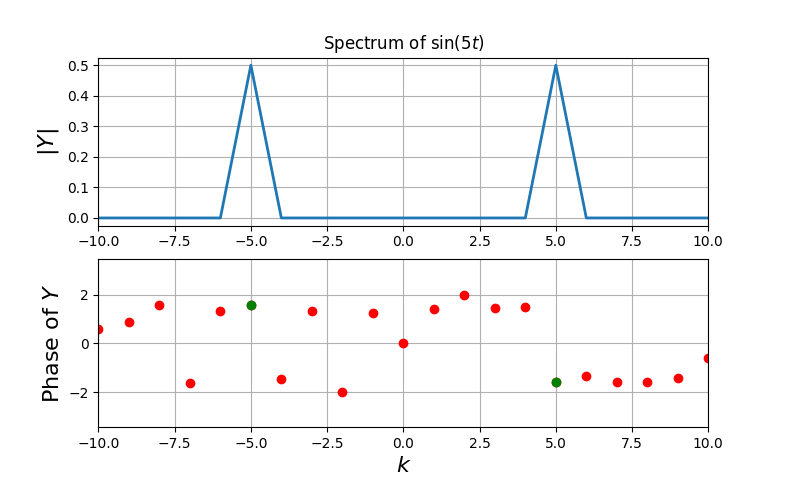
\includegraphics[width=0.8\textwidth]{Figure_1.png}
\end{center}
\section{Function 2 : $\left(1+0.1\cos\left(t\right)\right)\cos\left(10t\right)$}
$\left(1+0.1\cos\left(t\right)\right)\cos\left(10t\right)$ can be written as $$\left(1+0.1\cos\left(t\right)\right)\cos\left(10t\right) = \frac{e^{j10t} + e^{-j10t}}{2} + \frac{e^{j11t}+ e^{j9t} + e^{-j9t} + e^{-j9t}}{20}$$
Its Fourier Transform is $$Y(e^{j\omega}) = \pi (\delta(\omega - 10) + \delta(\omega + 10) + \frac{\delta(\omega - 9) + \delta(\omega + 9)}{20} + \frac{\delta(\omega - 11) + \delta(\omega + 11)}{20})$$
Its DFT would be same as Fourier Transform without the 2$\pi$ scaling $$Y(\omega) =  (\frac{\delta(\omega - 10) + \delta(\omega + 10)}{2} + \frac{\delta(\omega - 9) + \delta(\omega + 9)}{40} + \frac{\delta(\omega - 11) + \delta(\omega + 11)}{40})$$
So the DFT of this function will have 6 peaks at $\omega$ = -9,-10,-11 and 9,10,11 with peak value of 0.5 for $\omega$ = 10, -10 and 0.025 peak value for rest of the peaks. And phase at these points will be 0 as the transform is real.

\begin{lstlisting}[language=Python]
t=linspace(-4*pi,4*pi,513)
t=t[:-1]
y=sin(t)**3
Y=fftshift(fft(y))/512.0
w=linspace(-64,64,513);w=w[:-1]
figure()
subplot(2,1,1)
plot(w,abs(Y),lw=2)
xlim([-15,15])
ylabel(r"$|Y|$",size=16)
title("Spectrum of sin$^{3}$(t)")
grid(True)
subplot(2,1,2)
ii=where(abs(Y)>1e-6)
plot(w[ii],angle(Y[ii]),'go',lw=2)
xlim([-15,15])
ylabel(r"Phase of $Y$",size=16)
xlabel(r"$k$",size=16)
grid(True)
show()
\end{lstlisting}

The Output obtained is as predicted. The phase plot has some scattered points corresponding to the peaks but the scale of the plot is 10$^{-14}$  , which is practically 0.
\begin{center}
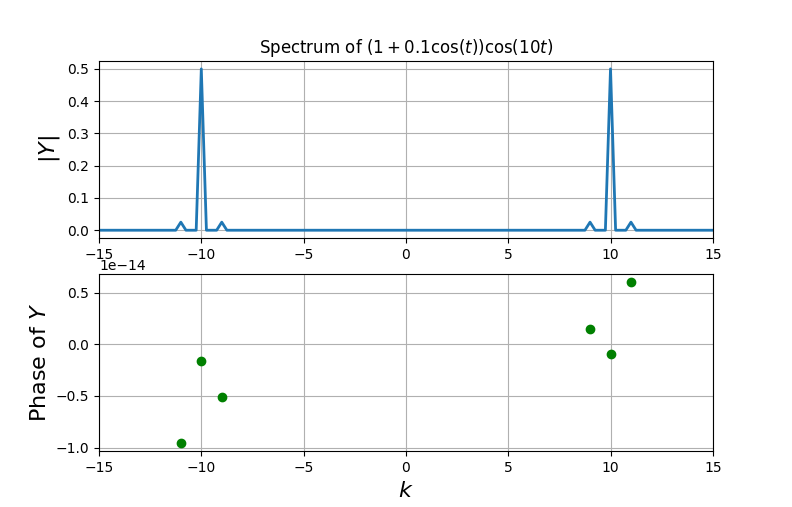
\includegraphics[width=0.8\textwidth]{Figure_2.png}
\end{center}


\section{Function 3 : sin$^{3}$(t)}
sin$^{3}$(t) can be written as $$ \frac{3sin(t) - sin(3t)}{4} $$
which can be written as $$sin(3t) = \frac{3}{8j}(e^{jt} - e^{-jt}) - \frac{1}{8j}(e^{j3t} - e^{-j3t})$$
Its Fourier Transform is $$Y(e^{j\omega}) = \frac{3\pi}{4j} (\delta(\omega - 1) - \delta(\omega + 1)) -  \frac{\pi}{4j} (\delta(\omega - 3) - \delta(\omega + 3))$$
Its DFT would be same as Fourier Transform without the 2$\pi$ scaling $$Y(\omega) = \frac{3}{8j} (\delta(\omega - 1) - \delta(\omega + 1)) -  \frac{1}{8j} (\delta(\omega - 3) - \delta(\omega + 3))$$

So the DFT of this function will have four peaks at $\omega$ = 1, -1, 3, -3 with peak value of 0.375 ($\frac{3}{8}$) for $\omega$ = 1,-1 and 0.125 ($\frac{1}{8}$) for $\omega$ = 3,-3. And phase at these points will be $\frac{-\pi}{2}$ at $\omega$ 1 and -3 and $\frac{\pi}{2}$ at $\omega$ -1 and 3.
\begin{lstlisting}[language=Python]
t=linspace(-4*pi,4*pi,513)
t=t[:-1]
y=sin(t)**3
Y=fftshift(fft(y))/512.0
w=linspace(-64,64,513);w=w[:-1]
figure()
subplot(2,1,1)
plot(w,abs(Y),lw=2)
xlim([-15,15])
ylabel(r"$|Y|$",size=16)
title("Spectrum of sin$^{3}$(t)")
grid(True)
subplot(2,1,2)
ii=where(abs(Y)>1e-6)
plot(w[ii],angle(Y[ii]),'go',lw=2)
xlim([-15,15])
ylabel(r"Phase of $Y$",size=16)
xlabel(r"$k$",size=16)
grid(True)
show()
\end{lstlisting}
The output obtained is same as predicted.
\begin{center}
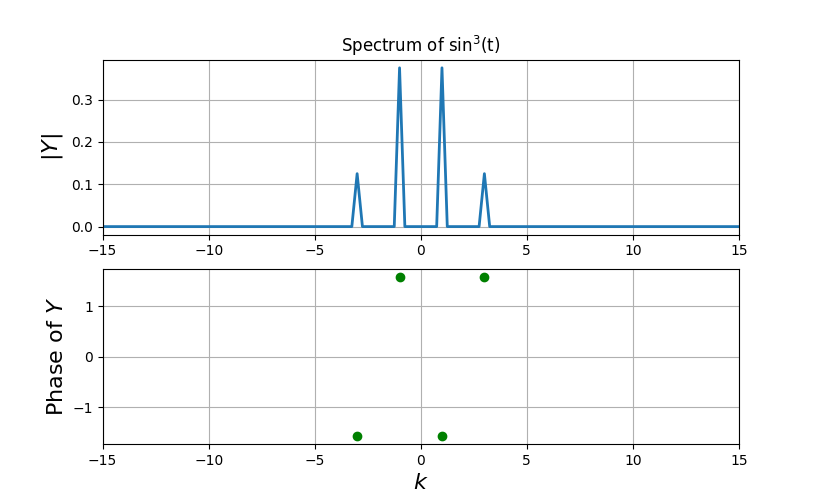
\includegraphics[width=0.8\textwidth]{Figure_3.png}
\end{center}

\section{Function 4 : cos$^{3}$(t)}
cos$^{3}$(t) can be written as $$ \frac{3cos(t) + cos(3t)}{4} $$
which can be written as $$cos(3t) = \frac{3}{8j}(e^{jt} + e^{-jt}) + \frac{1}{8j}(e^{j3t} + e^{-j3t})$$
Its Fourier Transform is $$Y(e^{j\omega}) = \frac{3\pi}{4j} (\delta(\omega - 1) + \delta(\omega + 1)) +  \frac{\pi}{4j} (\delta(\omega - 3) + \delta(\omega + 3))$$
Its DFT would be same as Fourier Transform without the 2$\pi$ scaling $$Y(\omega) = \frac{3}{8j} (\delta(\omega - 1) + \delta(\omega + 1)) +  \frac{1}{8j} (\delta(\omega - 3) + \delta(\omega + 3))$$

So the DFT of this function will have four peaks at $\omega$ = 1, -1, 3, -3 with peak value of 0.375 ($\frac{3}{8}$) for $\omega$ = 1,-1 and 0.125 ($\frac{1}{8}$) for $\omega$ = 3,-3. And phase at these points will be 0 as the transform is real.
\begin{lstlisting}[language=Python]
t=linspace(-4*pi,4*pi,513)
t=t[:-1]
y=cos(t)**3
Y=fftshift(fft(y))/512.0
w=linspace(-64,64,513);w=w[:-1]
figure()
subplot(2,1,1)
plot(w,abs(Y),lw=2)
xlim([-15,15])
ylabel(r"$|Y|$",size=16)
title("Spectrum of cos$^{3}$(t)")
grid(True)
subplot(2,1,2)
ii=where(abs(Y)>1e-6)
plot(w[ii],angle(Y[ii]),'go',lw=2)
xlim([-15,15])
ylabel(r"Phase of $Y$",size=16)
xlabel(r"$k$",size=16)
grid(True)
show()
\end{lstlisting}
The output obtained is same as predicted. The phase plot has some scattered point but the scale of the plot is 10$^{-15}$ hence it is practically 0.
\begin{center}
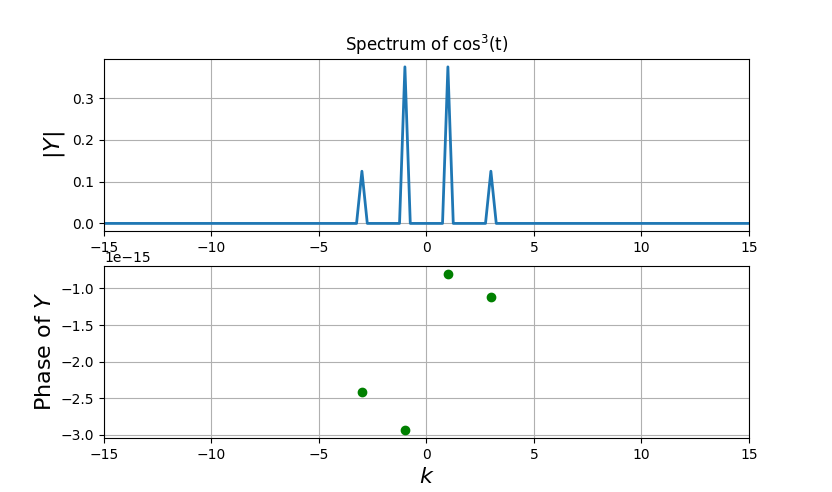
\includegraphics[width=0.8\textwidth]{Figure_4.png}
\end{center}

\section{Function 5: cos(20t + 5cos(t))}
cos(20t + 5cos(t)) is a Phase modulated signal . It has modulated wave of angular frequency 1 Rad/s and carrier of angular frequency 20 Rad/s.  $\omega$$_{c}$t + $\theta$$_{m}(t)$.
also $$A_{c}cos(\omega_{c}t + \beta si(\omega_{m}t)) = A_{c}re\{e^{j{\omega_{c}t}} e^{j\beta sin(\omega_{m}t)}\}$$
$$ = A_{c}re\{e^{j{\omega_{c}t}} 
\sum_{k=-\infty}^{\infty} J_{k}(\beta)e^{jk\omega_{m}t}\}$$
$$ = A_{c}re\{\sum_{k=-\infty}^{\infty}J_{k}(\beta)e^{j{\omega_{c}+k\omega_{m}}t}\}$$
$$ = A_{c} \sum_{k=-\infty}^{\infty}J_{k}(\beta)cos({\omega_{c}+k\omega_{m}}t)$$
where we used the fact that $ J_k(\beta)$ is real when $ \beta $ is real. From the equation it is clear that the sinusoidal PM spectrum consists of an infinite number of side-bands about the carrier frequency $ \omega_c$ (when $ \beta\neq 0$). The side bands occur at multiples of the modulating frequency $ \omega_m$ away from the carrier frequency $ \omega_c$. 

\begin{lstlisting}[language=Python]
t=linspace(-8*pi,8*pi,1025)
t=t[:-1]
y=cos(20*t + 5*cos(t))
Y=fftshift(fft(y))/1024.0
w=linspace(-64,64,1025)
w=w[:-1]
figure()
subplot(2,1,1)
plot(w,abs(Y),lw=2)
xlim([-30,30])
ylabel(r"$|Y|$",size=16)
title("Spectrum of cos(20*t + 5*cos(t))")
grid(True)
subplot(2,1,2)
ii=where(abs(Y)>1e-3)
plot(w[ii],angle(Y[ii]),'go',lw=2)
xlim([-30,30])
ylabel(r"Phase of $Y$",size=16)
xlabel(r"$k$",size=16)
grid(True)
show()
\end{lstlisting}
\end{lstlisting}
In the Output spectrum bands are observed which are centered at 20 Rad/s . Large number of spikes around it are obtained corresponding to the sidebands . The Phase spectrum has points with phase -$\frac{\pi}{2}$ , $\frac{\pi}{2}$ , -$\pi$ , $\pi$ and 0. Because can be decomposed into sine/cosine series with infinite harmonics.

\begin{center}
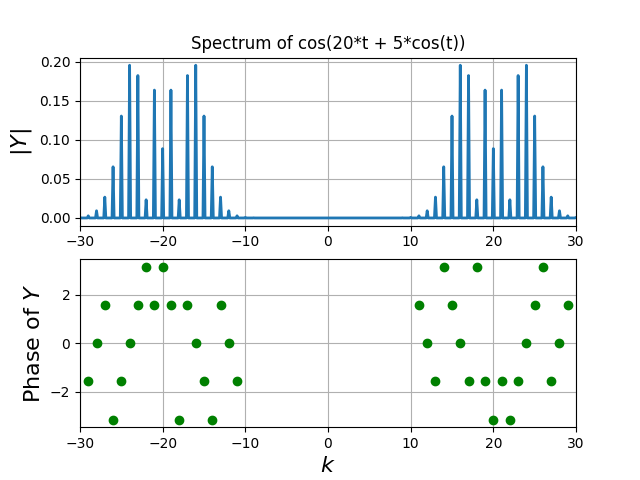
\includegraphics[width=0.8\textwidth]{Figure_5.png}
\end{center}

\section{Function 6 : $e^{\frac{-t^{2}}{2}}$}
The given Gaussian functions Discrete Fourier transform can not be obtained because it is not a band-limited signal . So only approximate DFT can be calculated. Taking a time scale for Pass high frequencies and High sampling Frequencies. Fourier Transform of a Gaussian is a Gaussian -
	$$x(t) = e^{\frac{-t^{2}}{2}} $$
    then,
    $$ X(j\omega) = \int_{\infty}^{\infty} f(t)e^{-\omega t}$$
    using f(t) = $e^{\frac{-t^{2}}{2}}$ its Fourier transform can be computed , easier way to do this is
    $$ f^{'}(t) = -tf(t)$$
taking Fourier transform on both the sides
	$$ j\omega F(j\omega) = -jF^{'}(j\omega)$$
Solving the differential equation above we get
    $$ F(j\omega) = Ce^{-\frac{\omega^{2}}{2}}$$
    $$C = F(0) = \int_{-\infty}^{\infty} e^{\frac{-t^{2}}{2}} = \sqrt[2]{2\pi} $$
    
So the DFT of this function is a Gaussian and is a real valued function and is always positive hence its phase is always 0.

To compare this with the expected CTFT we must multiply obtained DFT with 2T , where 2T is the period we defined for the Gaussian.

\textbf{Explanation} \#[4]\# line . After defining function it should be shifted in time domain to get correct phase. Here IFFTshift shifts the definition from 0 to 2*2$^{5}\pi$. Then we can take its FFT and again use FFTshift. Thus obtained transform need to be divided by number of samples and scaled by Time period. 
\begin{lstlisting}[language=Python]

t=linspace(-2**5*pi, 2**5*pi, 10001)	#for input e^(t*t/2) we will take time from 0 to 2pi
t=t[:-1]	#removing last value as it will be incuded in next period
y=exp(-t*t/2)	#input
Y = fftshift(fft(ifftshift(y)))*(2*(2**5*pi))/10000.0	#[4]#	 #computing fft and deviding by the scaling factor N.
w=linspace(-2**5*pi,2**5*pi,10001)
w=w[:-1]
figure()
subplot(2,1,1)
plot(w,abs(Y),lw=2)
xlim([-10,10])	#plotting magnitude response between -9000 and 9000
ylabel(r"$|Y|$",size=16)
title(r"Spectrum of $e^{-\frac{t^{2}}{2}}$")
grid(True)
subplot(2,1,2)
ii=where(abs(Y)>1e-6)
plot(w[ii],angle(Y[ii]),'go',lw=2)
xlim([-10,10])	#plotting phase response between -9000 and 9000
ylabel(r"Phase of $Y$",size=16)
xlabel(r"$k$",size=16)
grid(True)
show()
\end{lstlisting}
The output obtained is same as predicted. It is a Gaussian with phase oscillating between 0 and $\pi$.
\begin{center}
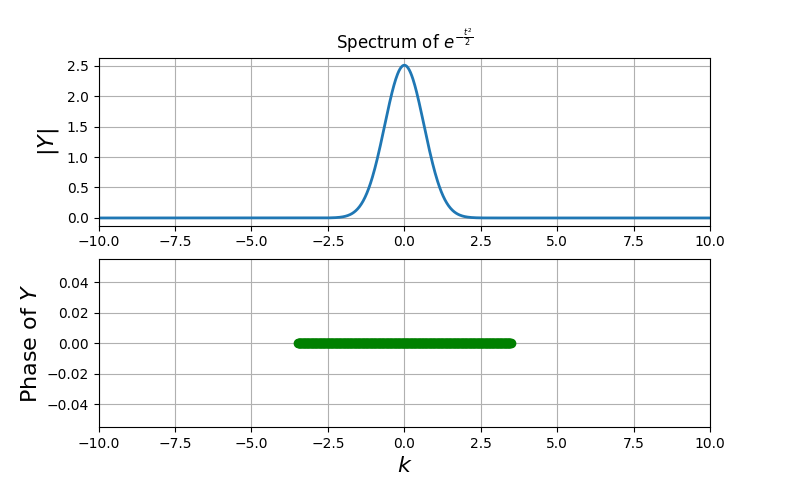
\includegraphics[width=0.8\textwidth]{Figure_7.png}
\end{center}
\subsection{Error Measurement}
Since the expected output is a Gaussian that is derived in previous section , To measure the accuracy of obtained DFT we will take absolute difference between obtained and expected DFT and change the time scale and sampling rate such that to obtain the difference in the order of 10$^{-6}$. To obtain this low error time scale is chosen from -2$^{5}\pi$ to 2$^{5}\pi$. and sampling rate 10000 samples/sec.

The Maximum absolute difference between the expected and obtained is 3.73910679856e-15.

\begin{lstlisting}[language=Python]
Y_exp = exp(-(w)**2/2)*sqrt(2*pi)
error =(abs(Y) - (Y_exp))
print max(error)
semilogy(w,error,'go')
show()
plot(w,abs(Y),'ro')
plot(w,Y_exp,'go')
legend(["obtained","expected"])
xlim([-10,10])
show()
\end{lstlisting}
The maximum absolute error obtained is in the orders of 10$^{-15}$. 
\begin{center}
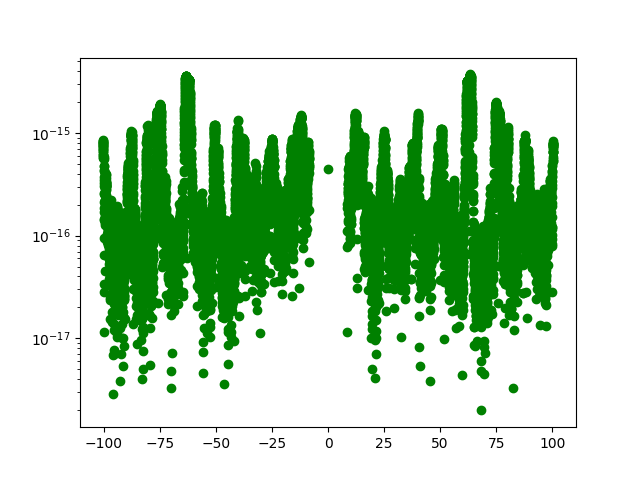
\includegraphics[width=0.8\textwidth]{Figure_8.png}
\end{center}

\end{document}

